% Chapter Template

\chapter{Introduction} % Main chapter title

\label{Chapter1} % Change X to a consecutive number; for referencing this chapter elsewhere, use \ref{ChapterX}


\section{Background}

Tracking a single object, given the location at the first frame, has been an ongoing challenge in the vision community for decades. Most recent approaches provide reasonably good performance~\cite{gao2022aiatrack,he2023target,yan2021learning,wei2023autoregressive,chen2023seqtrack}, especially when benchmarked on \emph{in-distribution (ID)} datasets, i.e., on the testing portion of the same datasets used for training. However, they incur high computational costs and hardware constraints, making their deployment ``in-the-wild'' in mobile, autonomous, and IoT applications still challenging.


\section{Current Challenges and Motivation}

The best-performing Transformer-based trackers operate between 0.4 to 4 frames per second (FPS) on a CPU~\cite{chen2023seqtrack,wu2023dropmae}, which is considered ``slower than real-time'' in many applications. Siamese tracking approaches provide the highest speed. FEAR-XS~\cite{borsuk2022fear} can operate at 100 FPS on a CPU, whereas an efficient Transformer-based approach, MixFormerV2-S\cite{cui2024mixformerv2}, operates at 37 FPS on a CPU. Despite the significant progress on efficient trackers, they still need to catch up when tested on \emph{out-of-distribution (OOD)} datasets, i.e., those that were not used during training.

A recently proposed benchmark, AVisT\cite{noman2022avist}, involves tracking objects under extreme visibility conditions that are common in-the-wild but not in most current training sets. High-performing tracking approaches tend to struggle when tested on AVisT, showing very significant performance deterioration. For instance, MixFormerV2-S exhibits remarkable performance with AUC of 58.7\% on an in-distribution benchmark like GOT-10k\cite{Huang2021}; however, it struggles on the OOD benchmark AVisT, with an AUC of 39.6\%. Therefore, the trade-off between the need of computational resources and \emph{OOD generalization} abilities of visual trackers is still unsatisfactory for their deployment in-the-wild under resource constraints.  


\section{Thesis Contribution}

\begin{figure}
    \centering
        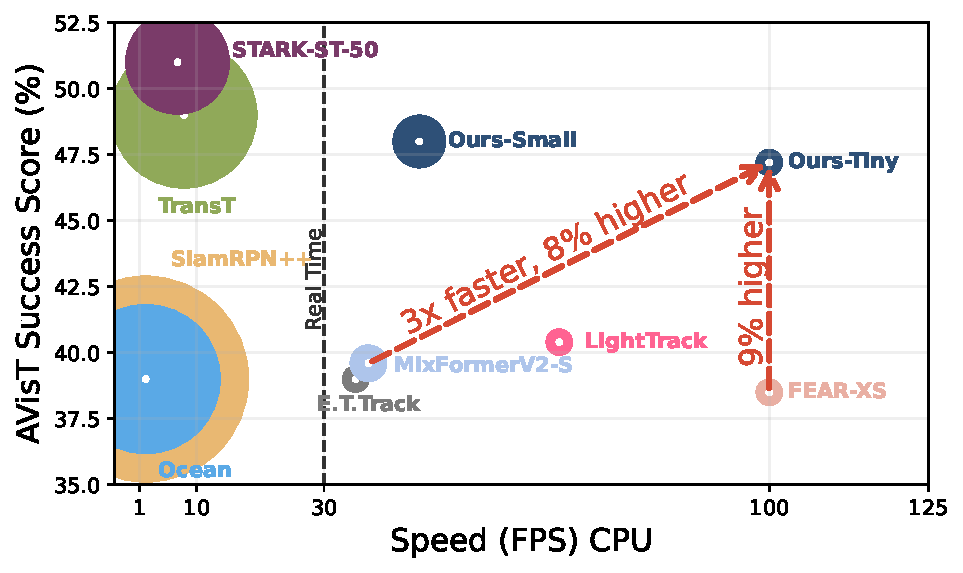
\includegraphics[width=1.0\textwidth]{figures/avist_comparison_fig_new.pdf}
    \caption{Comparison of our trackers with others on the AVisT~\cite{noman2022avist} dataset on a CPU. We show the success score (AUC) (vertical axis), speed (horizontal axis), and relative number of FLOPs (circles) of the trackers. Our trackers outperform other efficient trackers in terms of both speed and accuracy.}
    \label{fig:avist_comparision_fig}
\end{figure}

In this work we aim at significantly improving the trade-off mentioned above. We design a new Siamese tacker that preserves the high speed, reduced memory and computing requirements of the Siamese family while improving OOD generalization to near SOTA-level performance. From the architectural point of view, we make two key contributions. First, we better facilitate the visuo-temporal bridge between the static image template representing the target, and the search region image at current time. While~\cite{borsuk2022fear} popularized the use of a dual-template, which we also adopt, we introduce the use of a \emph{dual-search-region}. This will allow the tracker to stay anchored to the initial target representation while better latching onto its dynamic appearance variations. Second, we design a new learnable layer, the \emph{Fast Mixed Filtration}, that acts as an efficient filtration method for enhancing the relevant components of the combination of the representations forming the dual-template, as well as the dual-search-region. This is important because, given also the reduced representational capacity of smaller backbones used by efficient trackers, directly fusing the representations of the dual-template does not necessarily improve performance~\cite{borsuk2022fear}.


From the learning point of view we make two additional contributions. First, we introduce a new \emph{transitive relation loss} to help bridge the visuo-temporal similarities of the filtered representations of the dual-template and the dual-search-region, so that the relevant relational differences between them can be effectively leveraged for tracking purposes. Second, we more directly address the OOD generalization issue by tackling the dynamic distribution shifts while doing inference. As shown in many test-time adaptation (TTA) approaches for classification~\cite{wang2020tent,mirza2022norm, pan2018two, niu2022efficient, schneider2020improving, li2016revisiting}, shifts in Batch-Normalization (BN) statistics are majorly responsible for performance degradation under OOD testing. We introduce a \emph{dynamic TTA (DTTA)} approach specifically tailored to tracking. It is backward-free, thus lightweight computationally, and aims at dynamically updating the BN statistics while keeping them anchored to the source statistics. To the best of our knowledge this is the first work that uses TTA for single object visual tracking.


Combining the contributions above lead even our smallest and most efficient tracker, S-Tiny, to surpass relevant SOTA approaches on numerous benchmarks. Most notably, on the AVisT benchmark, S-Tiny achieves the AUC of 47.2\% while running at 100 FPS on a CPU, outperforming MixFormerV2-S by 7.6\% while being almost 3x faster. 
See \ref{fig:avist_comparision_fig}. 
An extensive set of experiments with multiple datasets and other approaches shows additional compelling results in support of our method.